\section{REST-for-Physics libraries}

\label{sec:libraries}
% We define the different libraries in REST with a short description. We dedicate a section to the detector library since it is a central library that connects raw, geant4, and track libraries. And since REST was born to be used in the domain of rare event physics we always need a detector, but we are not forced to use it.

The main framework contains common tools required for centralized data access, visualization, and basic analysis routines, including generic REST-for-Physics \emph{metadata} objects and \emph{processes} that do not require \emph{event} specialization, i.e. they only need to access information at the \emph{analysis tree} level. More specialized routines, requiring a dedicated \emph{event} data type, such as time signal processing or detector event reconstruction, are organized into libraries where all objects belonging to the library keep a closer relation and therefore enhanced connectivity.

A library is usually associated only to one or two \emph{specific event} types, increasing the connectivity between different \emph{specific event processes} inside the same library. This allows processes "living" inside a particular library to be connected at any order and combination inside a data processing chain within its library domain. A dedicated library, the \emph{connectors} library, hosts those \emph{specific event processes} or \emph{specific metadata} objects that need to interconnect different libraries, keeping all inter-library dependencies bounded together into a single entity, and allowing each library to be fully operational in stand-alone mode.

An object belonging to a particular library will be named after its library name as a prefix at the object name. Therefore, the \emph{TRest} naming convention is extended in the case of the libraries to \emph{TRestLibName}, helping us to promptly identify an object belonging to a particular library. In this context, we will continue highlighting the words that make reference to C++ objects using that pattern, such as \emph{TRestDetectorReadout} being written as \emph{detector readout}, or even omitting the library keyword, such as \emph{TRestDetectorGas} being written simply as \emph{gas}.

In spite of new libraries might be added in the future to the framework, this section briefly describes those fundamental libraries that gave REST-for-Physics enough functionality and versatility to be used in different aspects of rare event searches experiments.

\subsection{The detector library}

The detector library\,\cite{REST_Detector_Git} has been designed to be used for event reconstruction inside a Time Projection Chamber (TPC) filled with a gaseous medium\footnote{A liquid TPC or even other detector technologies could be exploiting common detection elements, as the generic \emph{detector readout} implementation, or other common detector physics processes. To date our code has been only exploited with gaseous TPCs.}. This library contains metadata objects that allow to define the detector configuration, such as the \emph{drift volume} description, the implementation of a \emph{detector readout} topology, or to provide access to particular \emph{gas} properties using the Magboltz interface implemented by \emph{Garfield++}. It also integrates processes implementing routines for event reconstruction from real detector data, and/or emulation of different physical response effects, such as including \emph{electron diffusion}, or introducing artificially the detector energy resolution by means of a \emph{smearing} process.

The \emph{readout} construction (see Figure\,\ref{fig:readouts}) is a crucial element on the detector library. This element has been designed to allow the definition of an arbitrary number of \emph{readout planes}, containing an arbitrary number of \emph{readout modules}, that are finally composed of physical \emph{readout channels} that identify unambiguously with the acquisition channels of an electronics setup. The \emph{readout channels} are at the same time built with \emph{readout pixels} which is the most basic element of a \emph{detector readout}. Such scheme allows us to create any arbitrary and complex topology, with the capability to efficiently translate - back and forward - physical coordinates and electronic channels for readouts containing few millions of pixels.

\begin{figure}[htb!]
  \centering
  \raisebox{-0.5\height}{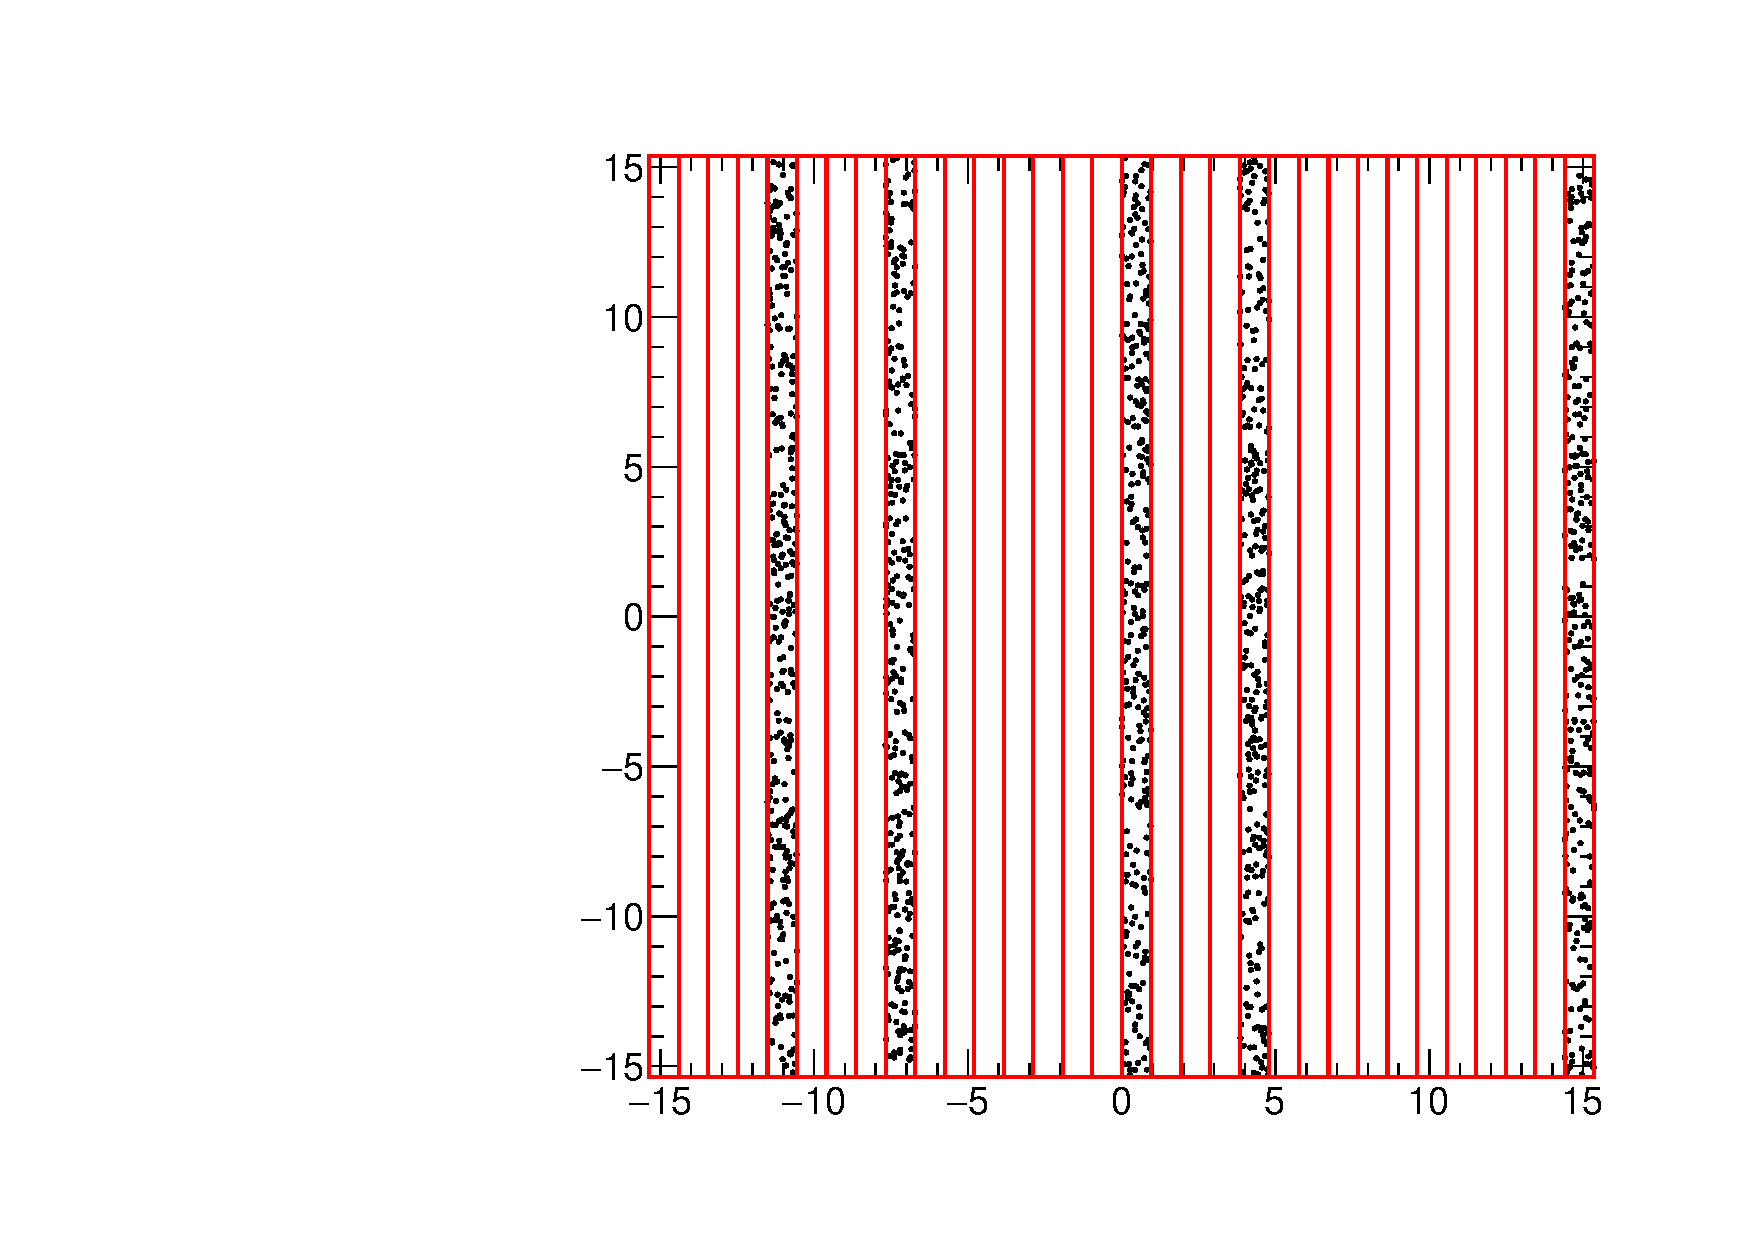
\includegraphics[width=0.33\textwidth]{images/stripped.pdf}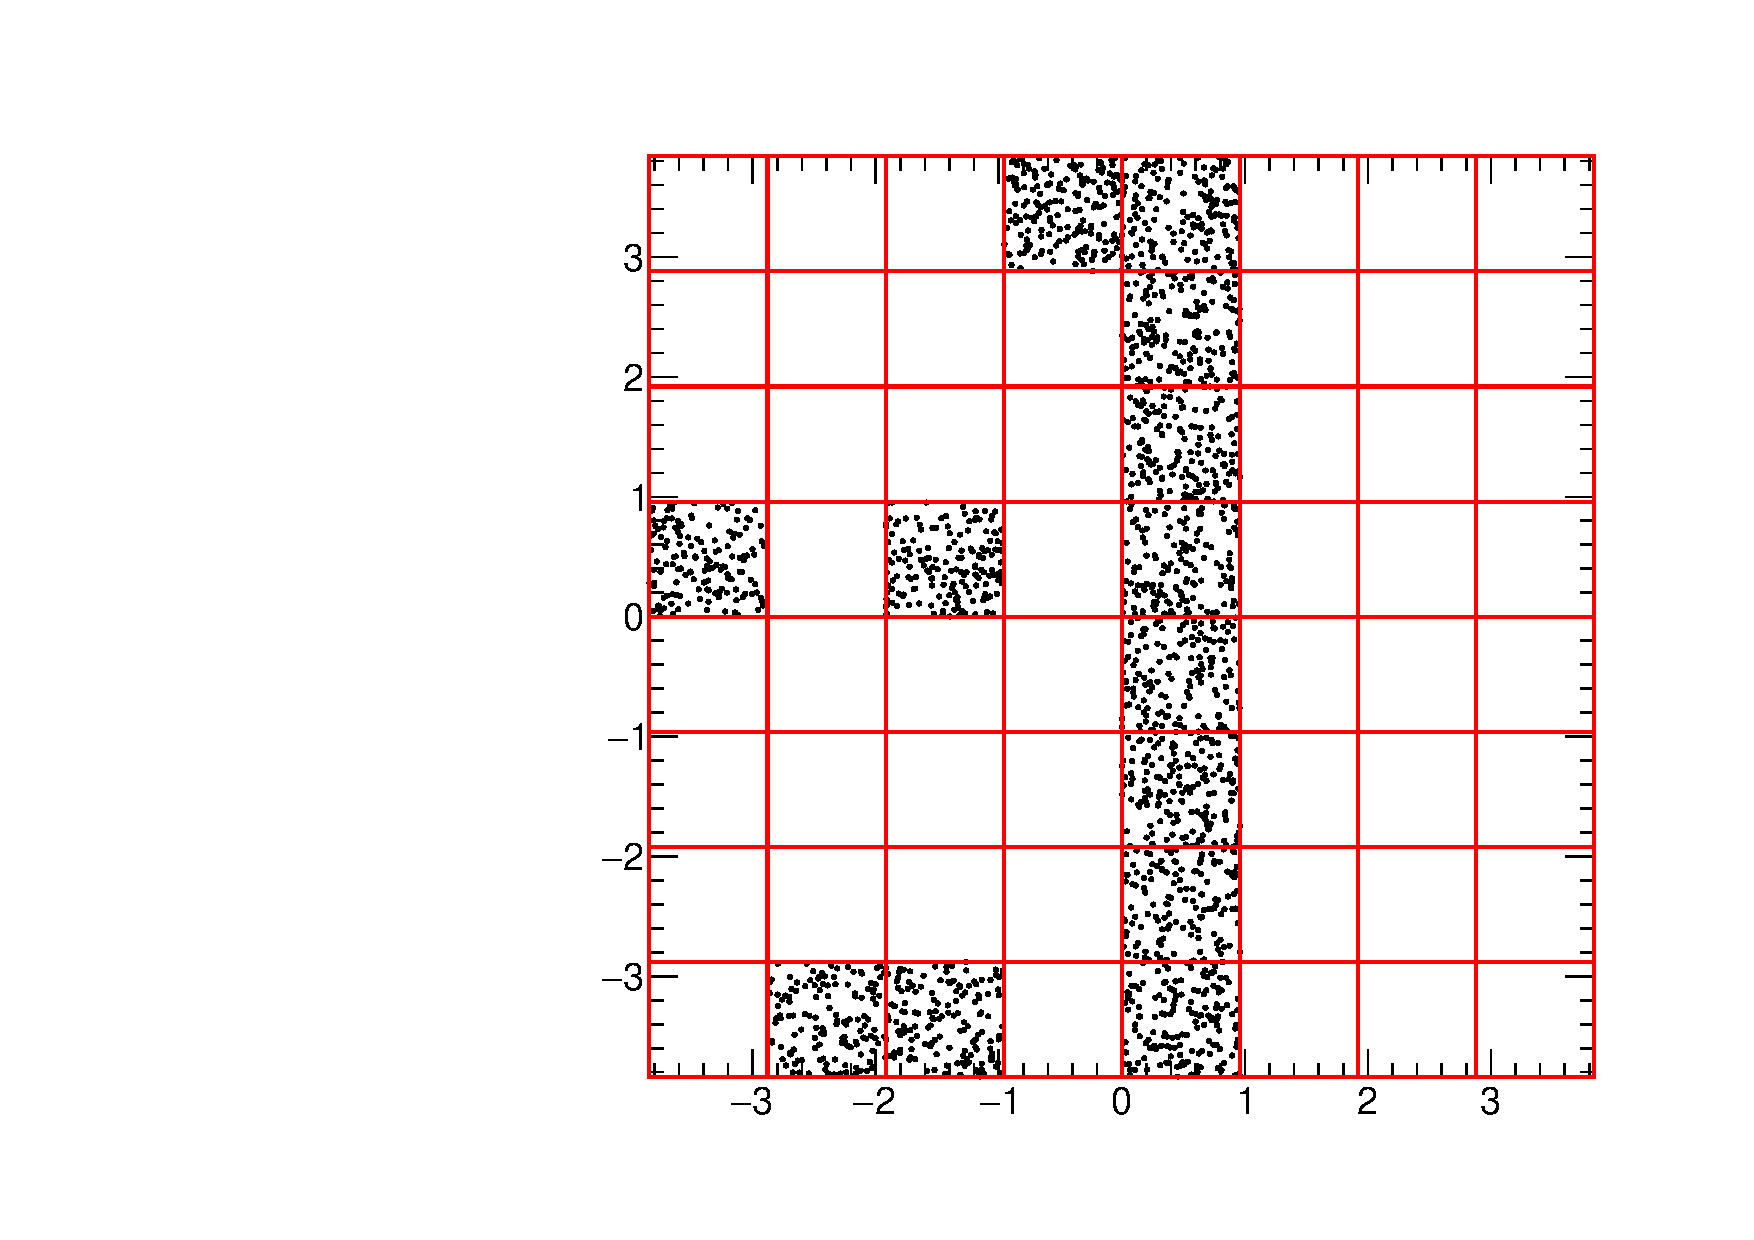
\includegraphics[width=0.33\textwidth]{images/pixel.pdf}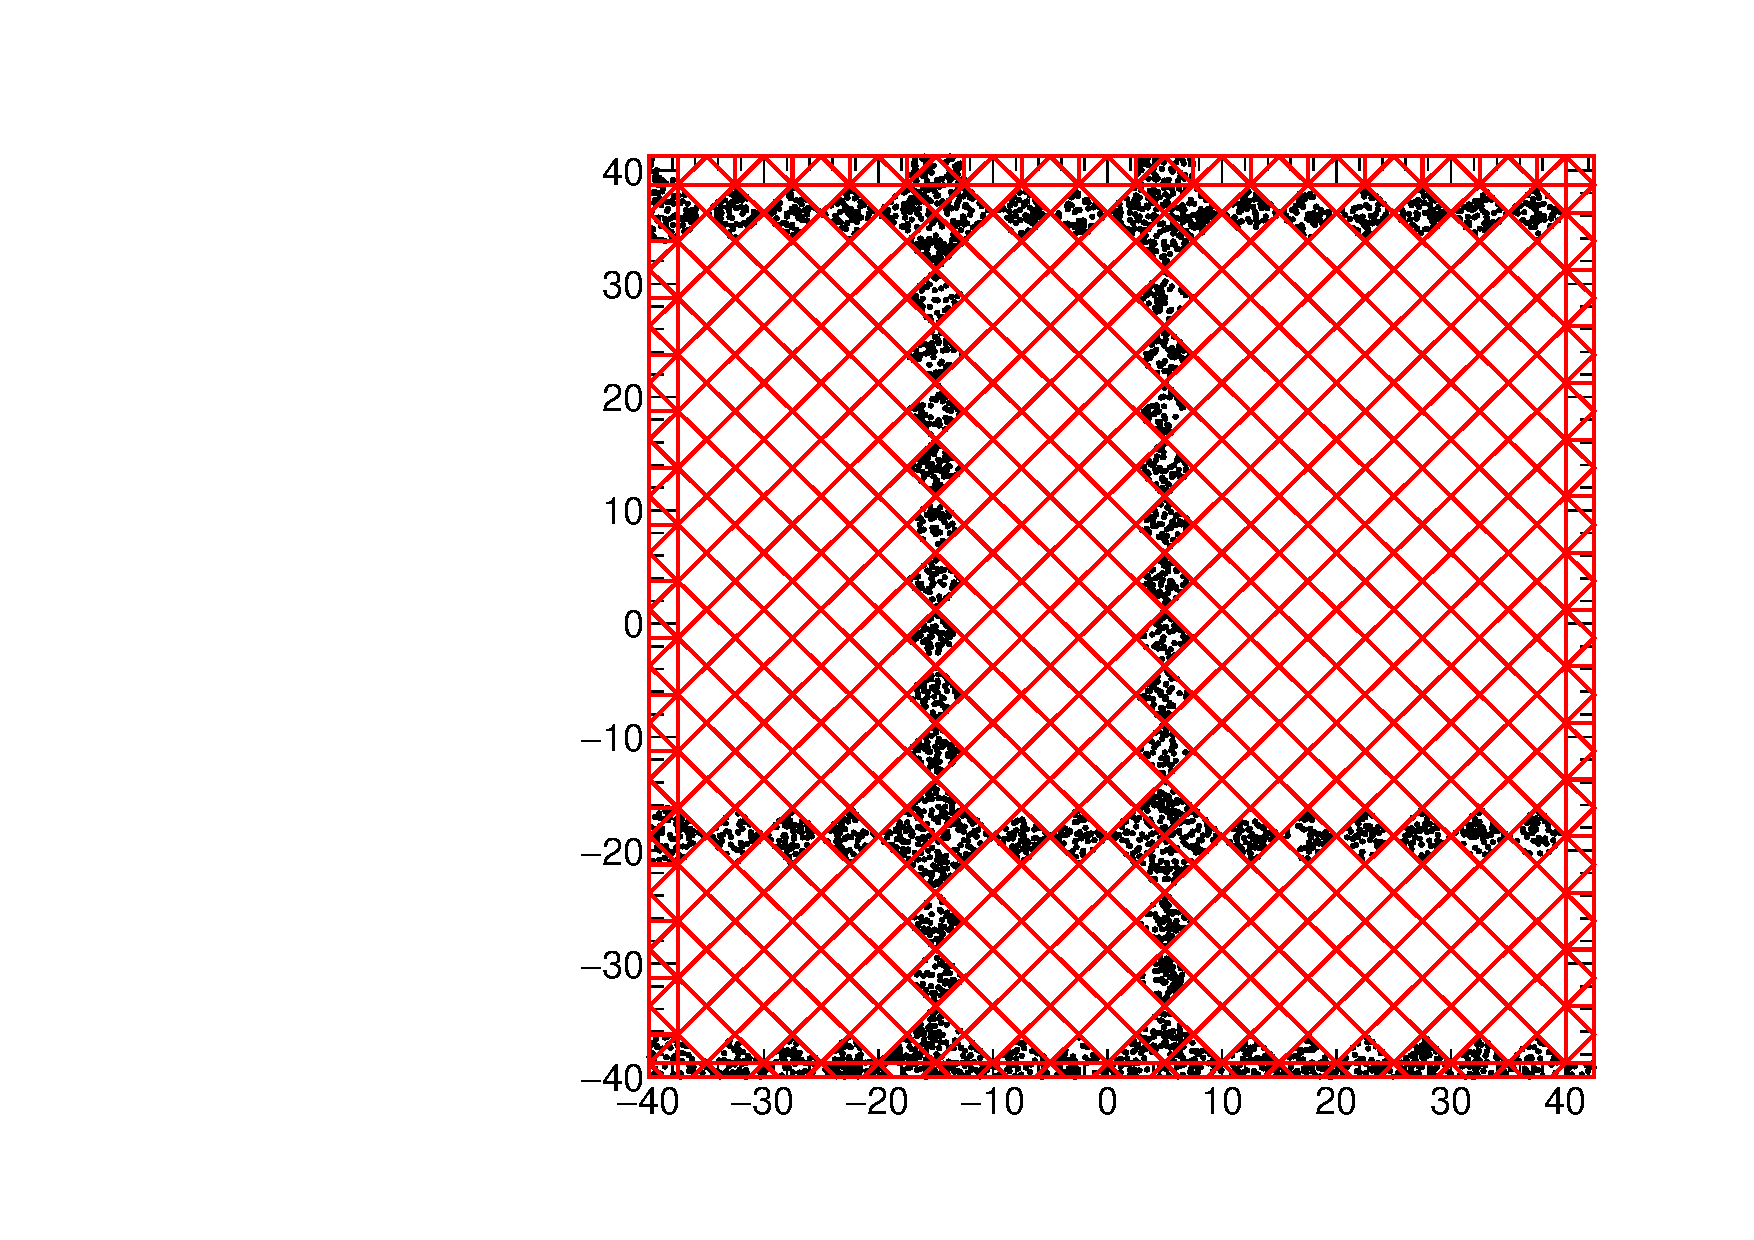
\includegraphics[width=0.33\textwidth]{images/microbulk.pdf}}
	\caption{Basic readout topologies that can be found at the \emph{basic-readouts} repository in REST-for-Physics. \emph{Left}, a stripped \emph{readout channel} layout. \emph{Middle}, a pixel \emph{readout channel} layout. \emph{Right}, a more complex \emph{readout channel} layout, being each \emph{channel}  composed by few interconnected \emph{readout pixels} that create a stripped pattern. The red lines represent the boundaries of the \emph{readout pixels}, while the black dots are produced randomly by Monte Carlo. In our validation routines we enable only few of the \emph{channels} to test the good behaviour of the \emph{detector readout} implementation.  }\label{fig:readouts}
\end{figure}

As any library, the detector library provides an event type to encapsulate the detector data. Up to date, and for convenience, it is the only library that defines two event types. The \emph{detector hits event} type, and the \emph{detector signal event} type. The \emph{hits event} allows to define a physical quantity, the energy deposits, at the detector physical volume, using a 3-dimensional spatial coordinate representation. The \emph{signal event} allows to describe the energy depositions as a function of the arrival time to the \emph{readout plane} associated to each detector electronics channel. The \emph{readout} implementation works as a dictionary between those two types, it is used to translate one event type into another by projecting the energy deposits into the \emph{readout channels}, or by recovering back the physical coordinate description from the readout channels information.

This library plays a central role on the description of the detector response and thus naturally includes connections to REST libraries related to raw electronics data processing (section\,\ref{sc:rawlib}), particle physics Monte Carlo event processing (section\,\ref{sc:geant4lib}), or physical track identification and pattern recognition routines (section\,\ref{sc:tracklib}). The processes allowing such library inter-connectivity are hosted at an independent library, the connectors library (see section\,\ref{sc:connectorslib}).

\subsection{The raw library}\label{sc:rawlib}

The raw library\,\cite{REST_Raw_Git} implements a \emph{raw signal event} type that is suited to describe the time evolution of physical quantities that have been acquired with a fixed sampling rate. Inside this event type we may find an arbitrary number of \emph{raw signals} that, in our case, are identified with the induced currents at the electronic channels of our detector. Each \emph{raw signal} inside event definition contains usually the same number of samples, a value which is fixed during the \emph{raw signal} initialization. The data depth of the physical quantity described inside the \emph{raw signal} is 16-bits precision, which is enough to fit the typical values of electronics acquisition systems.

This library includes processes related to signal conditioning, such as signal shaping, de-convolution, pulse fitting, de-noising, Fast Fourier Transform operations, common noise reduction, and other time signal manipulation routines (see Figure\,\ref{fig:rawlib}). 

\begin{figure}[htb!]
  \centering
  \raisebox{-0.5\height}{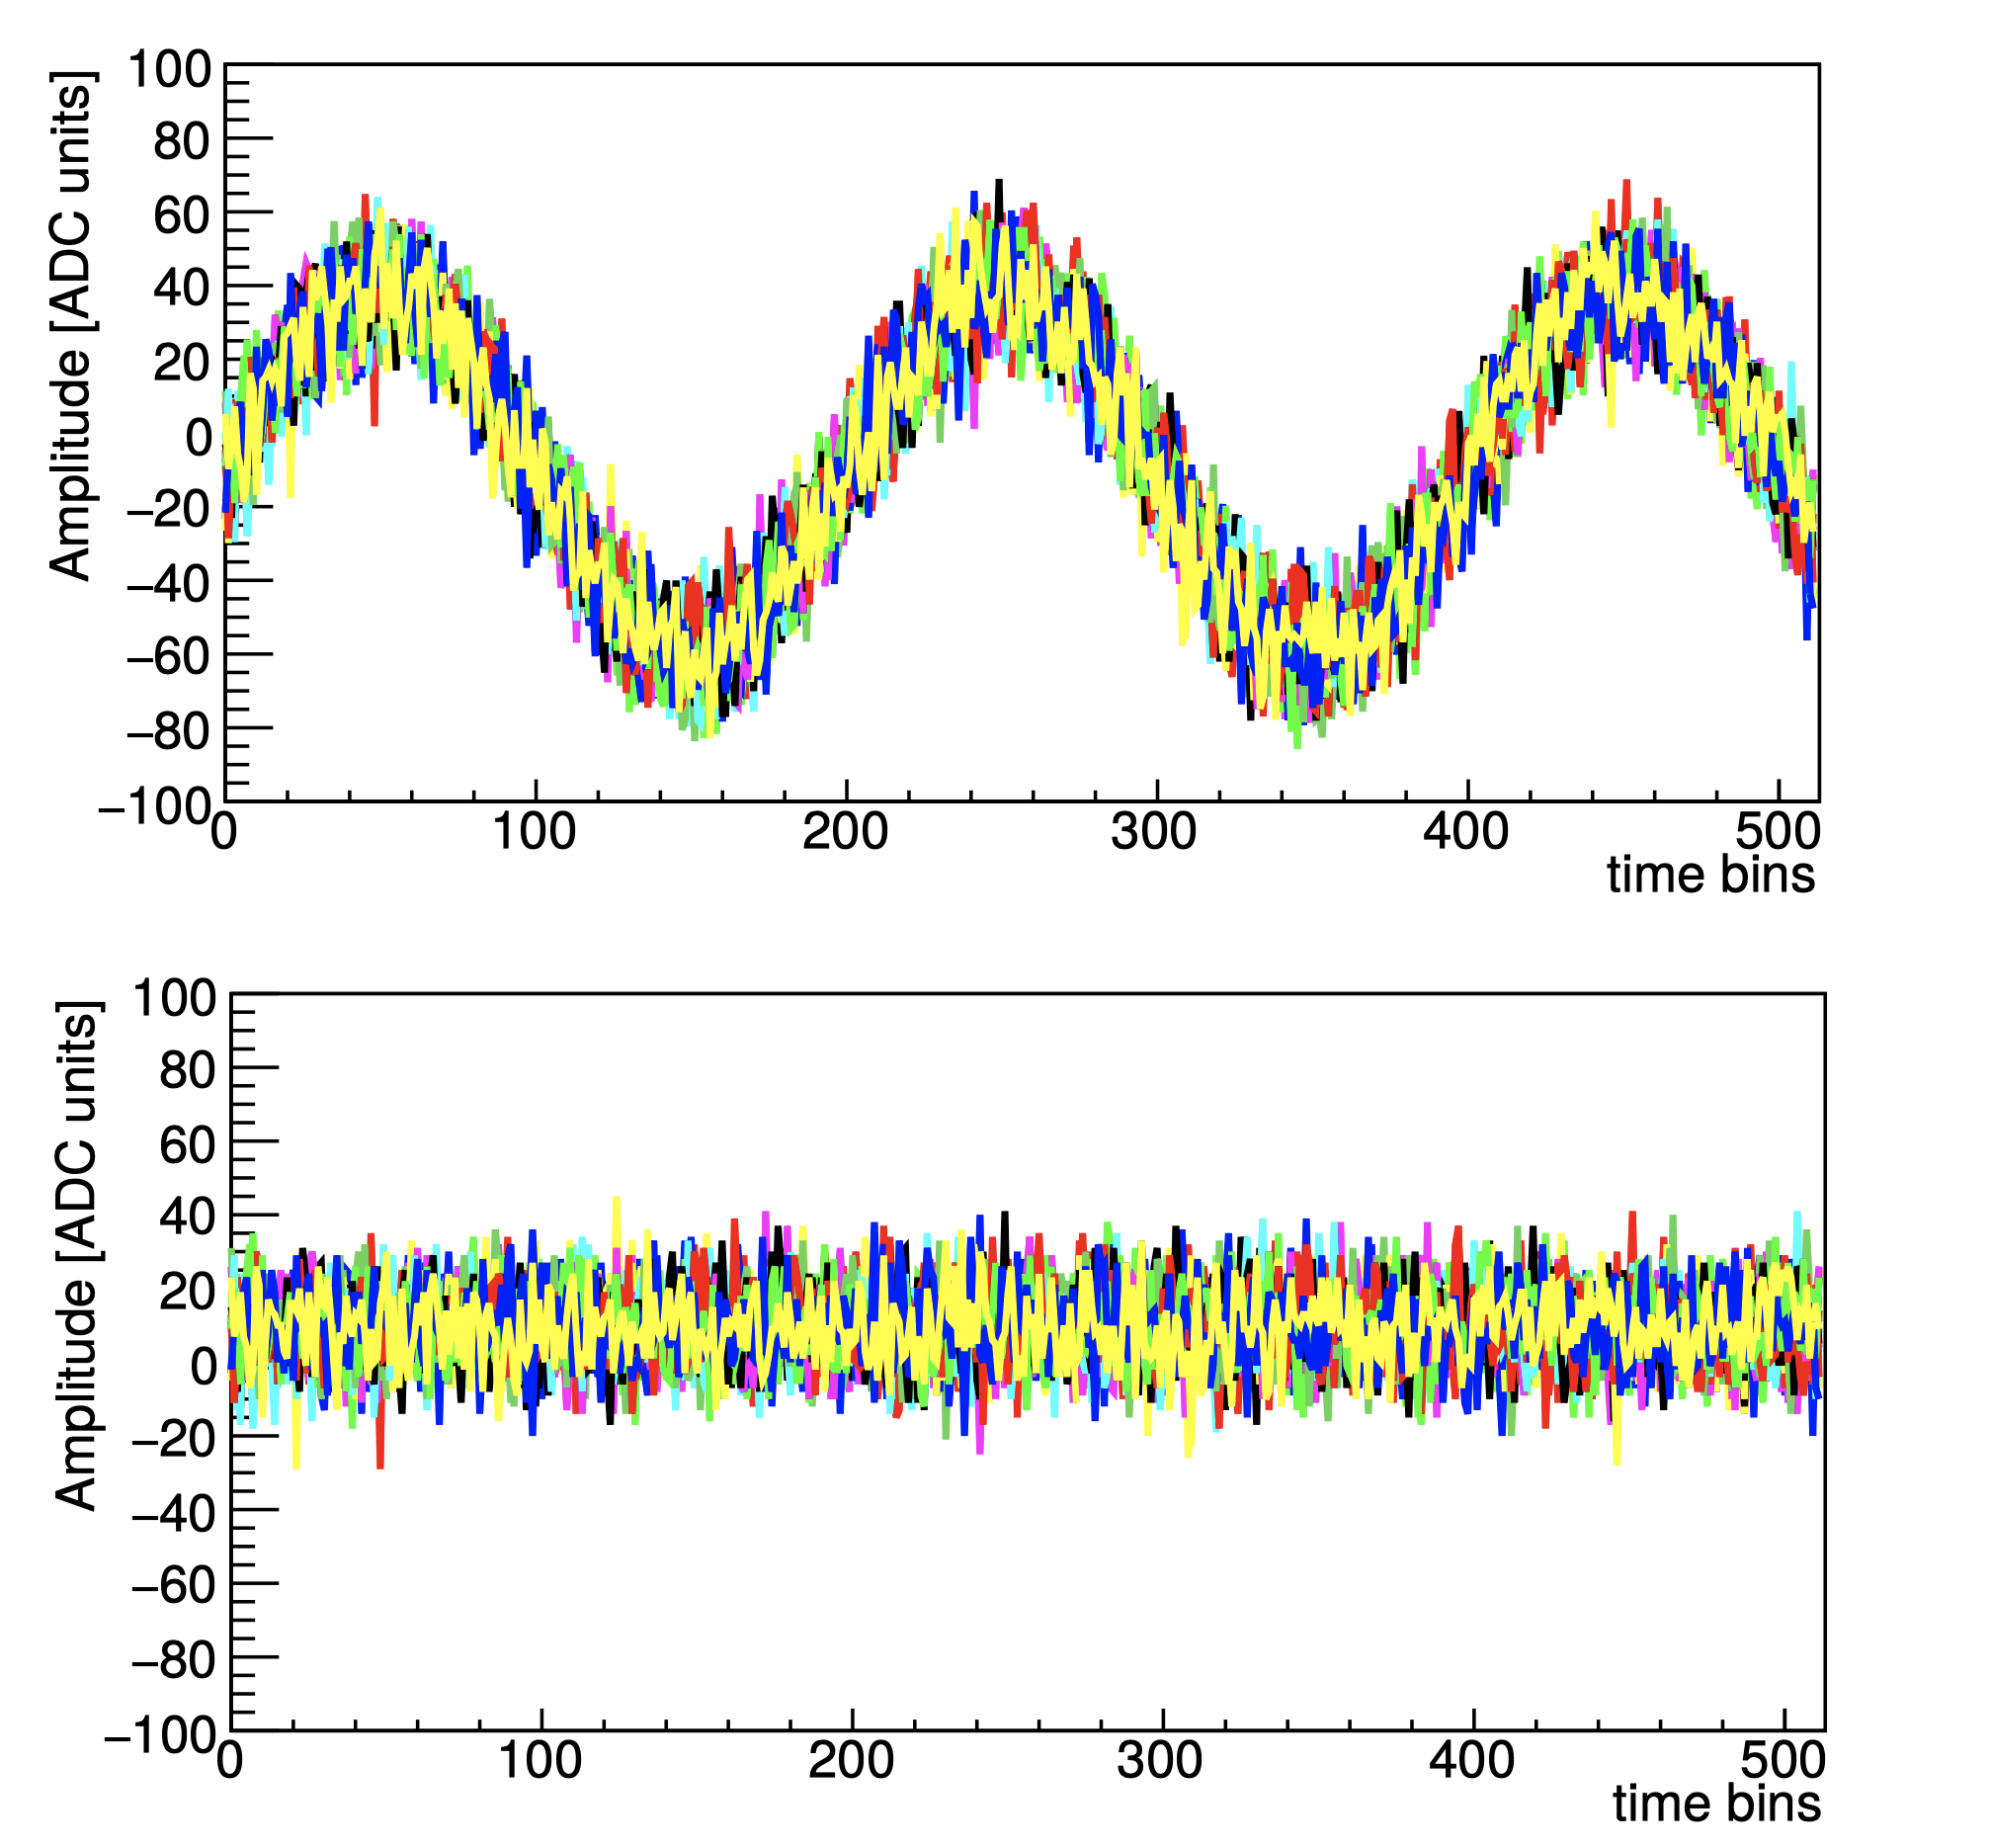
\includegraphics[width=0.27\textwidth]{images/commonNoise.png}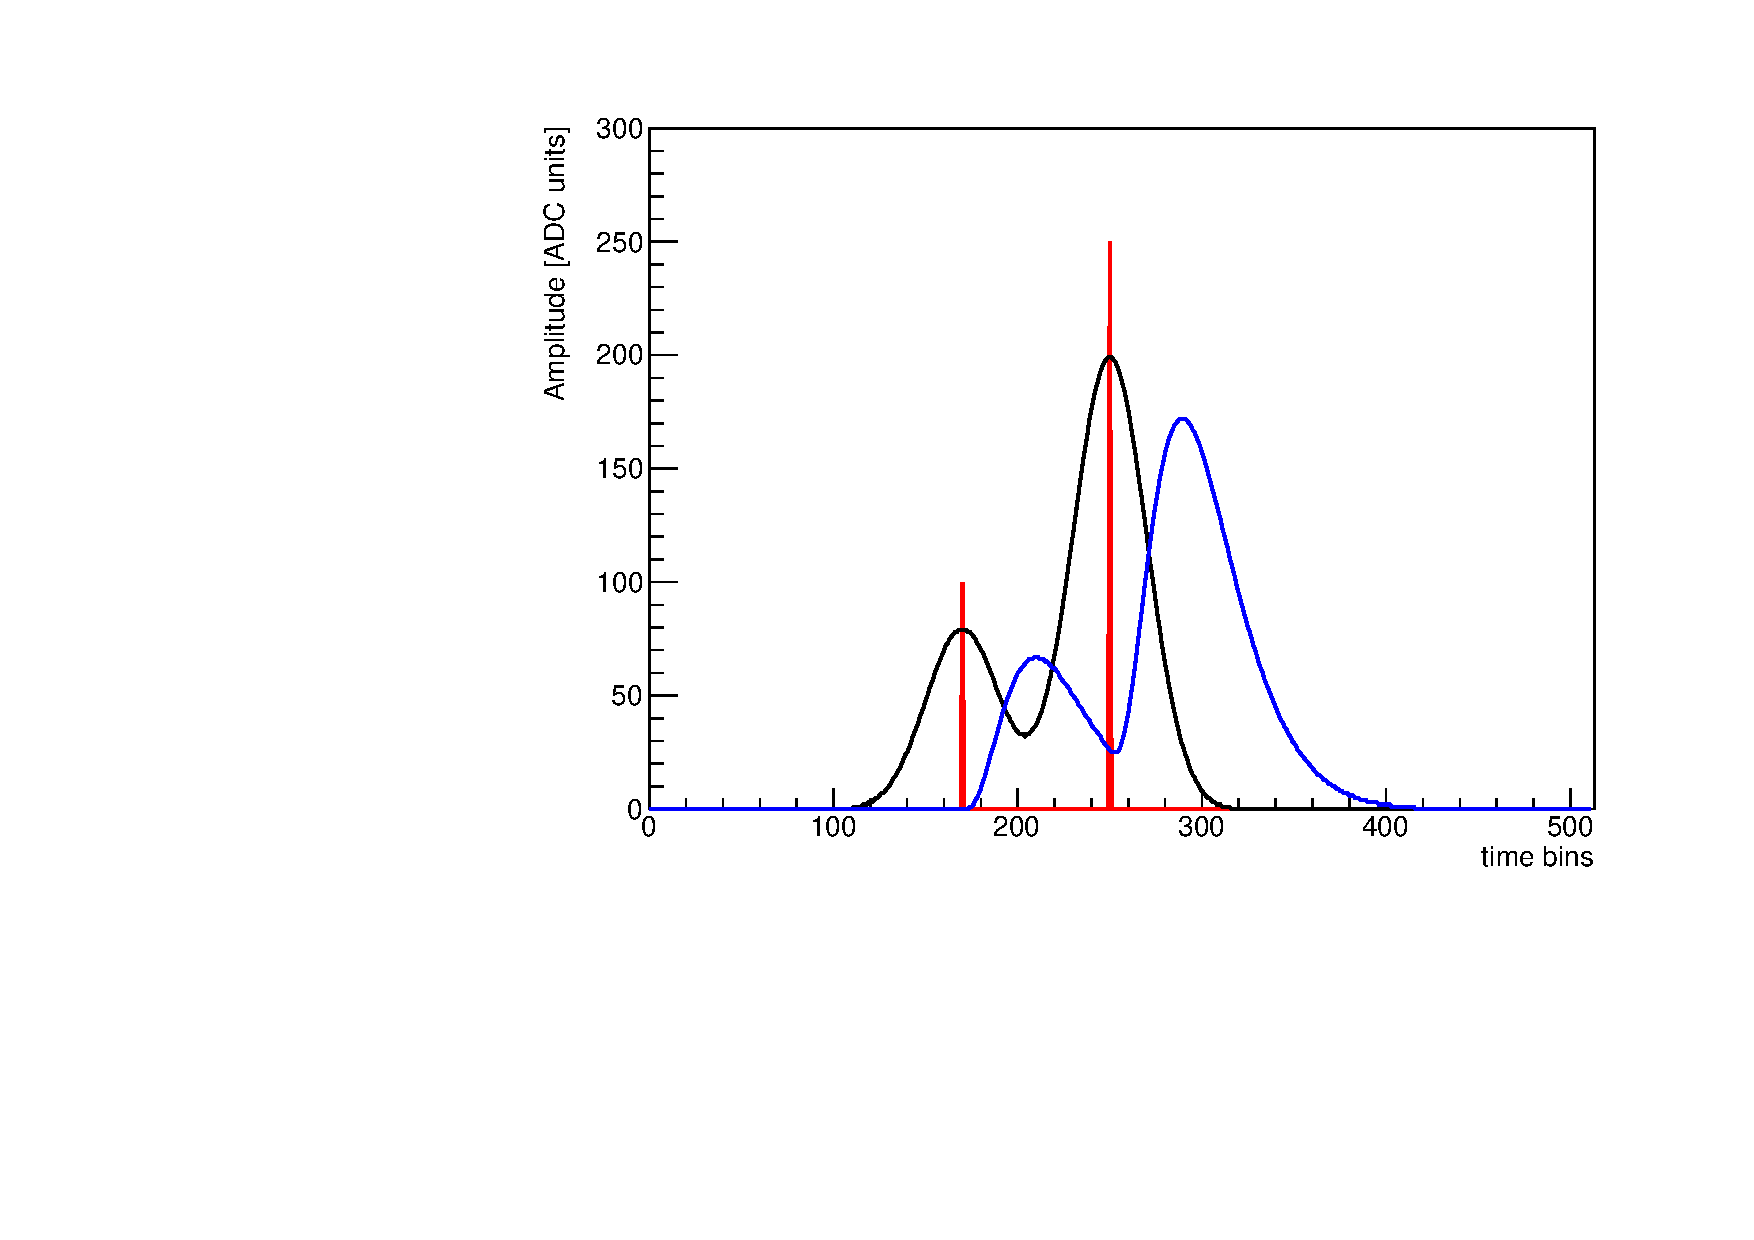
\includegraphics[width=0.37\textwidth]{images/shapingPlot.pdf}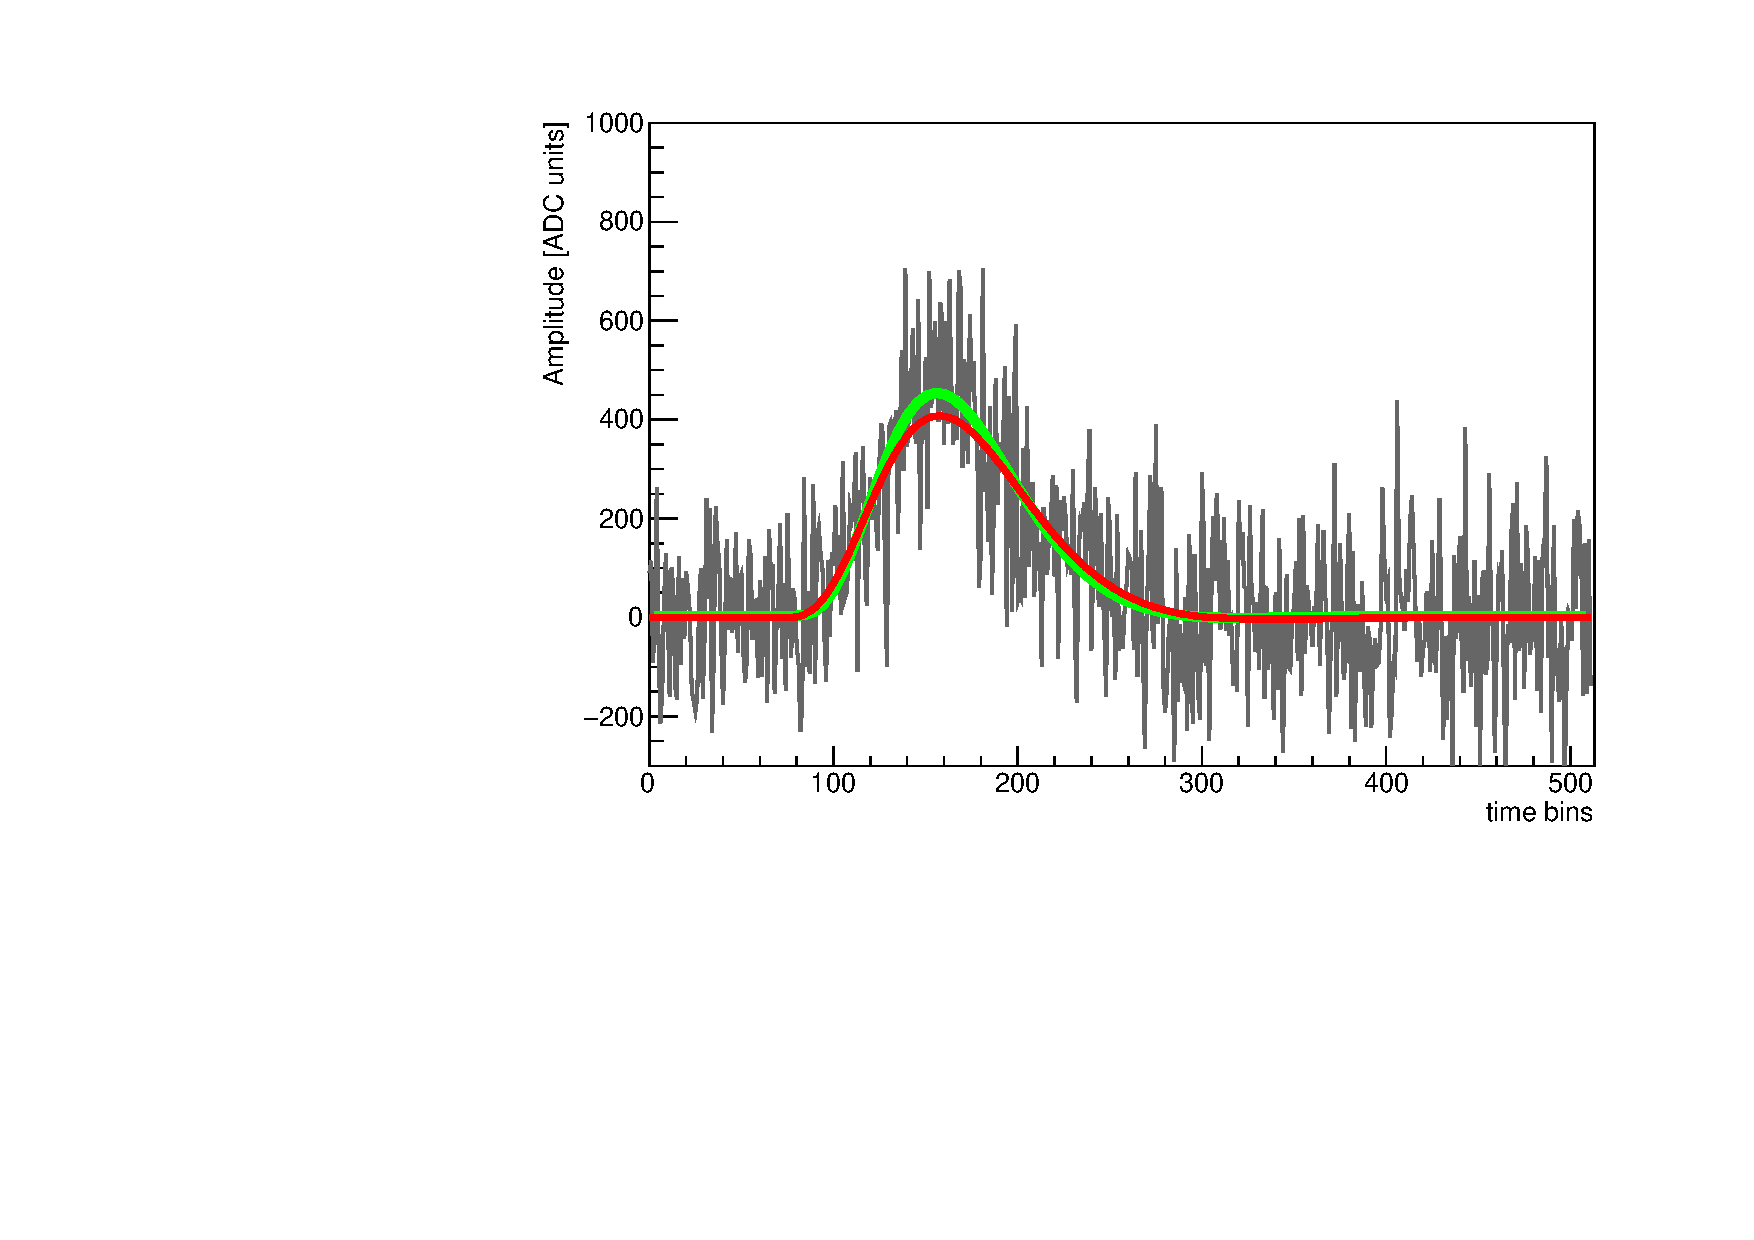
\includegraphics[width=0.39\textwidth]{images/fitComparison.pdf}}
	\caption{\emph{Left}, an artificially generated \emph{raw signal event} with a common sinusoidal pattern (top), and the result after applying the \emph{common noise reduction} process (bottom). Only randomly added noise remains. \emph{Middle}, an idealized \emph{raw signal} composed of 2-punctual deposits (in red) is conditioned by the \emph{shaping} process using a Gaussian (in black) and an AGET electronics response (in blue) convolutions. \emph{Right}, an artificially generated noise \emph{raw signal} (in black), together with the original pulse used to generate it (in red), and the recovered \emph{raw signal} after applying the \emph{fitting} process (in green).}\label{fig:rawlib}
\end{figure}

Apart from processes conditioning and manipulating a physical signal, the raw library includes processes, belonging to the \emph{external process} type, that allow to bring into the framework the binary data generated by different electronics acquisition cards used in our physics domain, such as AGET\,\cite{6154095} and AFTER chips, or Dream\,\cite{Dream} electronics, between others.

\subsection{The geant4 library}\label{sc:geant4lib}

The geant4 library\,\cite{REST_Geant4_Git} defines a \emph{geant4 event} type that registers the energy deposits, or hits, resulting from a \emph{Geant4} simulation. A \emph{Geant4} simulation performs the physics particle tracking including the interaction probability with the materials defined in a given detector geometry. The energy deposits are similar to those found at a \emph{detector hits event}, although the \emph{geant4 event} hits contain additional information, such as the physical interaction process, the geometrical volume where the interaction took place, or the remaining available kinetic energy of the particle that produced the energy deposit. The energy deposits, or hits, are encapsulated into \emph{geant4 tracks} that describe properties common to a particular group of hits, such as the particle name producing the depositions, the position where the particle was originated, the track and parent ids, and in general any relevant information directly extracted from the tracks produced by the \emph{Geant4} simulation package.

%Non-Geant4 dependency
It is important to mention that this library is not directly linked to the official \emph{Geant4} libraries. Its purpose is to store the event information generated by a \emph{Geant4} simulation, but once a simulation package has registered the information inside the \emph{geant4 event} data holder the connection to \emph{Geant4} libraries is not required anymore. In a different perspective, a user would be able to access a Monte Carlo database of previously \emph{Geant4} generated files in REST format without the need of performing a system \emph{Geant4} installation.

%restG4 GDML
Inside the REST-for-Physics ecosystem we have developed an independent package, \emph{restG4}\,\cite{REST_restG4_Git}, which is a particular \emph{Geant4} code implementation taking advantage of the \emph{geant4 event} type and all the definitions available at the library to describe the simulation conditions. Such as the \emph{geant4 metadata} object defining the number of primaries to be generated, together with their energy and angular distributions, or the generator type, in order to determine how the primaries will be launched or initialized. There are many other options that allow us to produce data sets at different experimental conditions, and define specific storage instructions. The library implements an additional metadata object, the \emph{geant4 physics list}, allowing to register and personalize the different particle physics processes that will be considered inside the simulation package. \emph{restG4} will register those metadata structures, and the \emph{geant4 event} tree, together with a \emph{run} metadata object complaining with the REST data format conventions so that the resulting data will be ready to be further processed with this or other libraries available in REST. A simulation with \emph{restG4} requires as input the description of those 3 objects, the \emph{run}, the \emph{geant4 metadata} and the \emph{geant4 physics list}, through a \emph{rml} file, and a description of the geometry through a GDML\,\cite{Chytracek:2006be} file (see Figure\,\ref{fig:geant4lib}).



\begin{figure}[htb!]
  \centering
  \raisebox{-0.5\height}{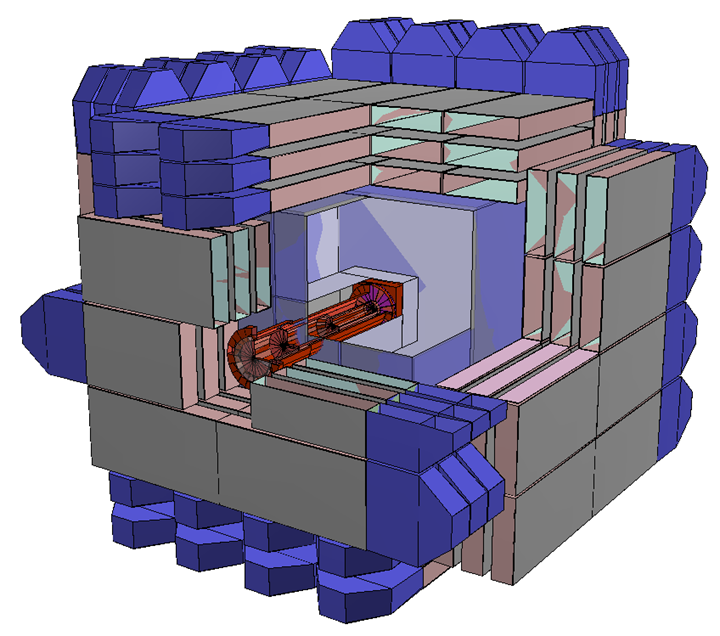
\includegraphics[width=0.4\textwidth]{images/BabyIAXO.png}\hspace{1 cm}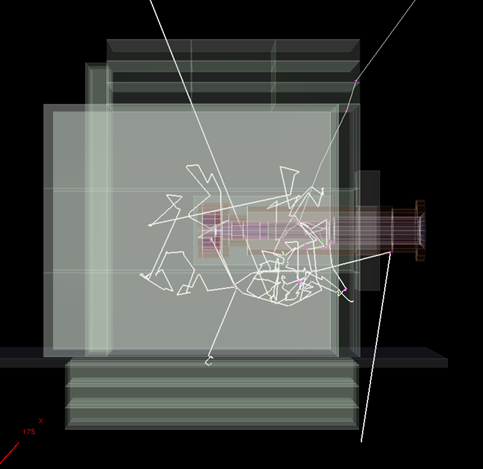
\includegraphics[width=0.35\textwidth]{images/neutron_event.png}}
	\caption{\emph{Left}, a visualization of the GDML geometry for the Baby-IAXO detector\,\cite{BabyIAXO:2020mzw}. \emph{Right}, a simulated cosmic neutron event at the same geometry visualized using the ROOT-Eve viewer. libraries.}\label{fig:geant4lib}
\end{figure}

%model
Once a first Monte Carlo data set has been generated using \emph{restG4} we will be able to process it using the existing routines at this library. These routines, or processes, might be used to extract the Monte Carlo truth at an early processing stage, such as the \emph{blob analysis} process allowing to extract the real electron track-ends at a $0\nu\beta\beta$ event, or the \emph{neutron tagging} process allowing to produce elaborated observables to perform a detailed analysis of the interaction of neutrons with an active cosmic veto system. In general, we will have available processes that may introduce sophisticated physics models which results will be introduced at the \emph{analysis tree} in the form of observables for being accessible at later processing stages. The main idea, or philosophy, is that \emph{restG4} is simply used to generate a first data set, while the geant4 library will be used to introduce models that need to know about the nature of the particles or the interactions that produced the energy depositions, such as it could be introducing offline energy corrections involving the particles quenching factor in the medium. Once all the relevant information has been extracted and placed in the form of observables at the \emph{analysis tree} we will be ready to migrate this data at other REST libraries (see section\,\ref{sc:connectorslib}) in order to include a detailed detector response, condition the data to mimic raw detector data, and perform the same data analysis processing we would do with real experimental data.

\subsection{The track library}\label{sc:tracklib}

The track library\,\cite{REST_Track_Git} implements a \emph{track event} type allowing to define inheritance relations between a set of \emph{tracks} stored inside the event. A \emph{track} itself contains a group of hits (or cluster) that define a discrete energy distribution in a 3-dimensional coordinate space. In order to produce, or initialize a first \emph{track event}, a process at the connectors library (section\,\ref{sc:connectorslib}) allows to use the \emph{detector hits event} as input to identify groups of hits, or energy deposits, that have a proximity relation in order to create \emph{tracks}. It is important to remark that the \emph{track event} is an abstract object\footnote{Not to be confused with an abstract c++ class. Notice that it would have been highlighted otherwise. We want to emphasize that it is an object that has not a strict or fixed scope.} that allows to define groups of hits, clusters, with a inheritance relation, i.e. we may develop \emph{track} levels by generating new daughter \emph{tracks} from the original ones. This could be exploited in different contexts, it could serve to describe random isolated clusters (or group of hits) in a single physical volume, or to describe correlated \emph{tracks} at independent physical volumes by creating a new \emph{track} that includes all those mother tracks into one.

This library contains graph theory algorithms helping to identify and reconstruct physical tracks by finding the shortest path that interconnects energy deposits within a \emph{track}, and processes that allow to extract topological information from a \emph{track event}. Since graph theory algorithms are computationally expensive when dealing with a large number of nodes, we need to previously include a \emph{reduction} process to decrease the effective number of \emph{hits}, so that we are able to apply Travelling Sales Problem (TSP) algorithms in an acceptable computation time. TSP methods help to find a reasonable solution for the physical track identification, although we usually need to apply further \emph{reconnection} algorithms to improve the result (see Figure\,\ref{fig:tracklib}). These algorithms become crucial on the identification of neutrino less double beta decays ($0\nu\beta\beta$), being their implementation at \emph{tracklib} motivated to address the topological event discrimination at the PandaX-III experiment\,\cite{Galan:2019ake}.

\begin{figure}[htb!]
\centering
    \raisebox{-0.5\height}{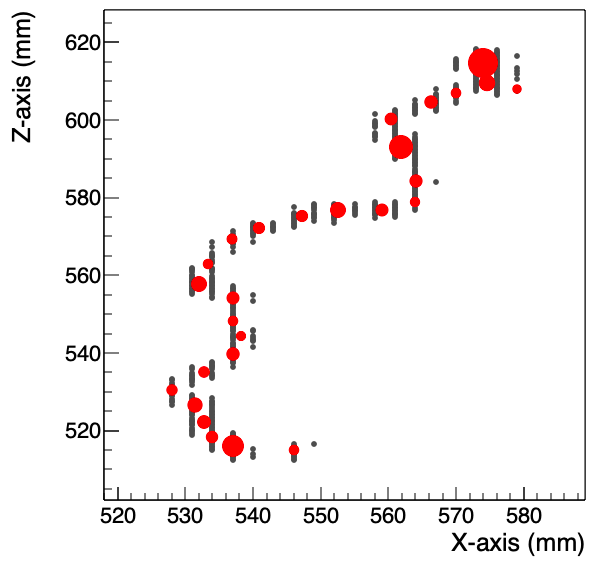
\includegraphics[width=0.33\textwidth]{images/TrackReduction.png}
    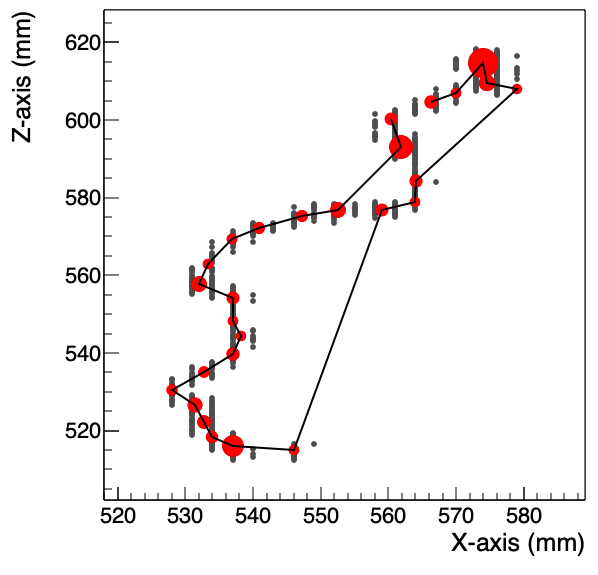
\includegraphics[width=0.33\textwidth]{images/TrackMinimized.png}
    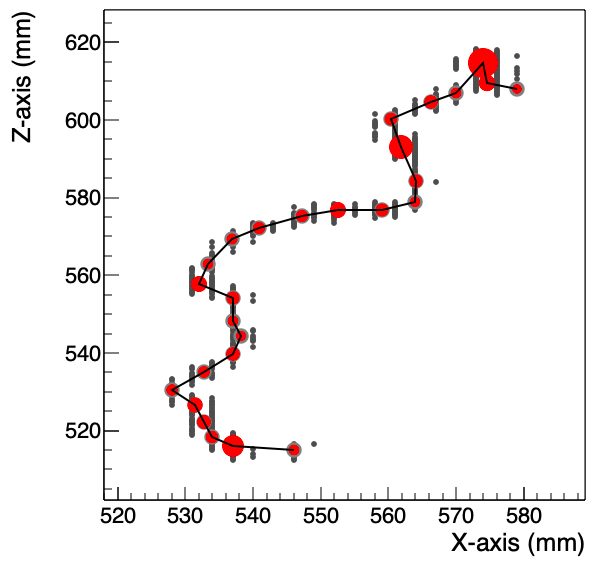
\includegraphics[width=0.33\textwidth]{images/TrackReconnected.png}}
    \caption{A \emph{track event} representation of a simulated $0\nu\beta\beta$ decay after the treatment with different \emph{track} processes used for physical track identification. \emph{Left}, an image of the hit reduction produced by the \emph{track reduction} process. The red circles represent the final position of reduced hits, which size is weighted with their energy value. The small grey circles on the background represent the hits of the \emph{parent track} used as input. \emph{Middle}, a polyline is added to this representation to visualize the hits inter-connectivity after the \emph{track path minimization} process. If path minimization works on the whole, it produces at times obviously unphysical connections, as our example illustrates. \emph{Right}, the unphysical connections are corrected using a \emph{track reconnection} process. Figure extracted from reference\,\cite{Galan:2019ake}.}
    \label{fig:tracklib}
\end{figure}

\subsection{The connectors library}\label{sc:connectorslib}

The connectors library\,\cite{REST_Connectors_Git} contains objects that need to combine the features from objects residing at different REST-for-Physics libraries. This includes processes that transform the \emph{event} type from one library specific \emph{event} type into another library \emph{event} type. Or it includes complex \emph{metadata} object descriptions that require to combine specific metadata descriptions from different libraries. The main mission of this library is to keep inter-library dependencies isolated or encapsulated at a single entity, allowing the fundamental libraries described in previous sections to be operative in a stand-alone mode philosophy (see Figure\,\ref{fig:connectorslib}). The REST-for-Physics building system will compile only those connectors library objects related to libraries that were marked for compilation, and in the extraordinary case that only a single library was marked for compilation, the connectors library will not be compiled at all. This library differentiation helps on the coherent development for the given purpose a particular library was designed for. Using this design any library may be enabled or disabled at will, avoiding unnecessary dependencies on dedicated systems.

\begin{figure}[htb!]
  \centering
  \raisebox{-0.5\height}{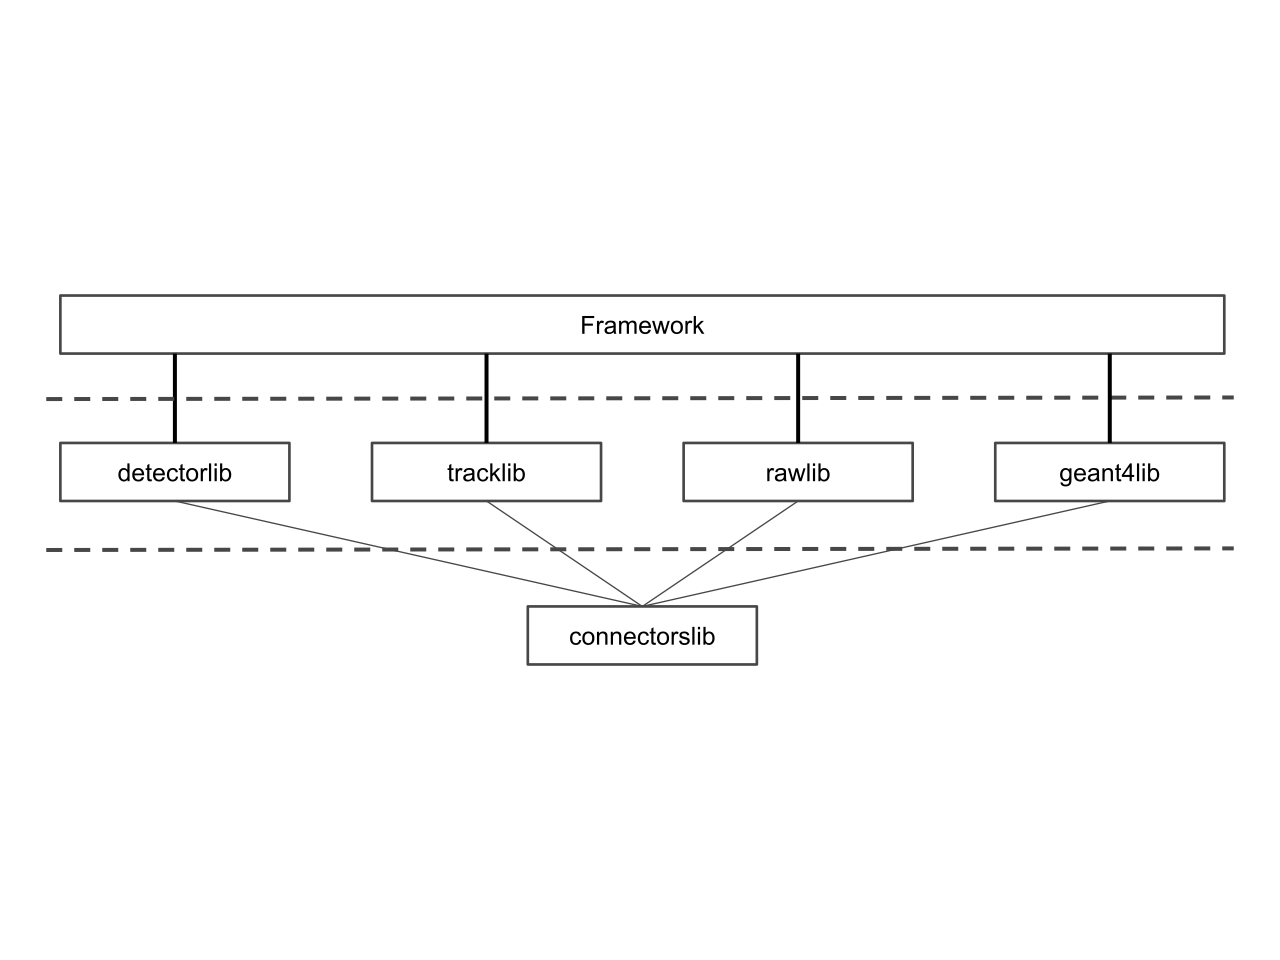
\includegraphics[trim=0 130 0 130, clip, width=0.75\linewidth]{images/connectorslib_new.png}}
	\caption{REST-for-Physics libraries hierarchy and connectivity to the framework. The connectors library depends on the other fundamental libraries, providing objects that help inter-library communication. On the other hand, fundamental libraries with a direct connection to the framework are capable to operate in a stand-alone mode, without any other REST-for-Physics libraries requirements.}\label{fig:connectorslib}
\end{figure}

Thus, the main functionality of this library is to allow jumping from one fundamental library domain into another, such as transforming a \emph{raw signal event} into a \emph{detector signal event} by using data reduction techniques or grouping hits at a \emph{detector hits event} to produce a \emph{track event}. However, the connectors library must not be understood as a simple \emph{event} data type transformation, since the \emph{specific event} data usually requires sophisticated routines including the detector physics involved for the event reconstruction, data reduction inside signal processing algorithms, or graph theory for the clustering of hits . This library will play a crucial role to define how different library domains inter-connect.


%contains active routines

%not only i.e. hit clustering to transform detector hits into a track event, or raw signal to be transformed into a detector event. It also may contain other complex processes that require to use 2 libraries simultaneously.